%!TEX root = ../main.tex

\graphicspath{{./figures/chapter5/}}

\chapter{RNA localization by the numbers}
\label{ch:chapter5}

\minitoc
\newpage

In this chapter, I present several applications of the pipeline described in the previous chapters.
More specifically, I analyze experimental datasets in order to explore, quantify and validate biological insights about \ac{mRNA} localization.
Results from this chapter are computed from three different high content screening studies, totaling tens of genes observed through thousands of bioimages.

In the first section, I describe the development of a general classification pipeline to identify generic \ac{mRNA} localization patterns from \ac{smFISH} images~\cite{CHOUAIB_2020}.
In the second section, exploiting the same dataset, I focus on a specific and novel clustering pattern: translation factories.
These first two sections describe the work published in:

\begin{center}
	\color{green}
	R. Chouaib, A. Safieddine, et al. (2020), \textit{A dual protein-mRNA localization screen reveals compartmentalized translation and widespread co-translational RNA targeting}, Developmental Cell 54 (6), 773.
\end{center}

In the third section, we used a \ac{GFP} channel to visualize and detect centrosomes.
I observed a centrosomal localization patterns for different transcripts and mitosis phases~\cite{safieddine_choreography_2021}.
This work was published in:

\begin{center}
	\color{green}
	A. Safieddine, E. Coleno, et al. (2021), \textit{A choreography of centrosomal mRNAs reveals a conserved localization mechanism involving active polysome transport}, Nature Communications 12 (1), 1352.
\end{center}

In the fourth section, I detail several transcripts with a localization to cellular protrusions~\cite{pichon_kinesin_2021}.
This last section mainly describes results presented in:

\begin{center}
	\color{green}
	X. Pichon, K. Moissoglu, et al. (2021), \textit{The kinesin KIF1C transports APC-dependent mRNAs to cell protrusions}, RNA 27 (12), 1528.
\end{center}

\section{A systemic quantification of RNA localization}
\label{sec:general_pattern_recognition}

In~\cite{CHOUAIB_2020}, I implemented a quantitative pipeline to analyze the localizations of \ac{mRNA} molecules.
This work lays the foundation of the Python packages developed in FISH-quant v2~\cite{Imbert_fq_2022}.
My contribution consists in classifying individual cells with one or several \ac{RNA} localization patterns.

\subsection{Introduction}
\label{subsec:introduction_general_pattern}

Most of \ac{mRNA}s have a random distribution throughout the cytoplasm, but some localize in specific subcellular regions~\cite{Blower_2013, Jung_2014, Eliscovich_2017, Bovaird_2018}.

Such localization can be related to either \ac{RNA} metabolism, for example with untranslated \ac{mRNA}s stored and repressed in \ac{P-bodies} (but not degraded~\cite{Hubstenberger_2017}), or  protein metabolism with locally translated proteins.
This local synthesis concerns both mature proteins and nascent peptides.
Different cellular processes imply the delivery of mature proteins in specific subcellular regions and a local regulation of the proteome.
Local translation can contributes to cell fate determination during metazoan development, as observed in~\cite{melton_translocation_1987} with a clear modification of the Vg1 \ac{RNA} spatial distribution between mature and immature Xenopus oocytes.
In mammalian cells, \ac{RNA} localization influences cell polarization and motility, usually through actin localization at the cell edge~\cite{Lawrence_1986}.
Locally translated proteins are also known to be involved in axonal growth and so neural plasticity~\cite{VanDriesche_2018}.
Finally, by precisely controlling the \ac{mRNA} localization and the subsequent translation process, cells can avoid to release proteins at inappropriate places~\cite{Muller_myelin_2013} and help the synthesis of protein complexes~\cite{pichon_visualization_2016}.

Several mechanisms drive the localization of \ac{mRNA}s.
Sometimes the nascent peptide can serve as a targeting signal, but most of the time the \ac{RNA} molecule itself will initiate its localization.
The molecule often include a zip-code sequence that is read by a \ac{RBP} and starts the assembly of a transport complex comprising different organelles or motor proteins.
Such complex can then directly transport the \ac{RNA} along the cytoskeleton~\cite{Blower_2013}.
Coupled with an anchoring mechanism at the targeted destination, it provides a better stability of the \ac{RNA} localization.
Following a random diffusion across the cell, a transcript can also be trapped in specific subcellular compartments.
Likewise, a local protection from degradation will bias the \ac{RNA} spatial distribution.

In a pioneering work on Drosophila embryogenesis~\cite{lecuyer_global_2007}, authors analyze 3,370 genes and find that 71\% of them encode a transcript with a non-uniform localization pattern.
In human cell lines recent studies exploit and improve \ac{smFISH} techniques to image thousands of \ac{mRNA}s in the perinuclear region, the mitochondria and the cell membrane~\cite{battich_image-based_2013, Chen_2015, eng_seqfish_2019, Xia_2019}.
In~\cite{CHOUAIB_2020}, we explored more systematically the link between non-random \ac{RNA} localization and local translation in HeLa cells.
We performed a quantitative analysis leveraging supervised and unsupervised methods in order to recognize up to 6 different localization patterns.
The current section emphasizes this quantitative pipeline that contributes to make our analysis scalable and more robust.

\subsection{Materials and methods}
\label{subsec:materials_general_pattern}

The quantitative pipeline used in this study and the existing work in FISH-quant v1 are the building blocks of FISH-quant v2.
Therefore, the various methods presented here were not yet packaged in \emph{bigfish}, but Python libraries that formed its foundation were already in used.
This work was developed in Python and the code repository is public\footnote{\url{https://github.com/Henley13/paper_translation_factories_2020}}.

\subsubsection{Experimental data}

The study is a dual-color screen, where all genes were GFP tagged, to measure the protein, and the same oligos, targeting the GFP sequence, were used for the \ac{smFISH}.
Our collaborators first manually inspected 500 genes to identify potential transcripts with non random localization patterns.
To obtain a more quantitative description of these data, we also developed a pipeline to systematically classify \ac{RNA} localization patterns.
To this end, I exploited a dataset of 526 \ac{FoV}s, consisting of 3D stacks (z-spacing of 0.3$\mu$m) with DAPI and \ac{smFISH} as illustrated in Figure~\ref{fig:fov_racha}.
Acquisitions were performed with a Zeiss Axioimager Z1 widefield microscope or a Nikon Ti fluorescence microscope.
In total, this dataset was built from 57 independent experiments gathering observations from 27 different \ac{mRNA}s under different experimental conditions.

\begin{figure}[]
    \centering
    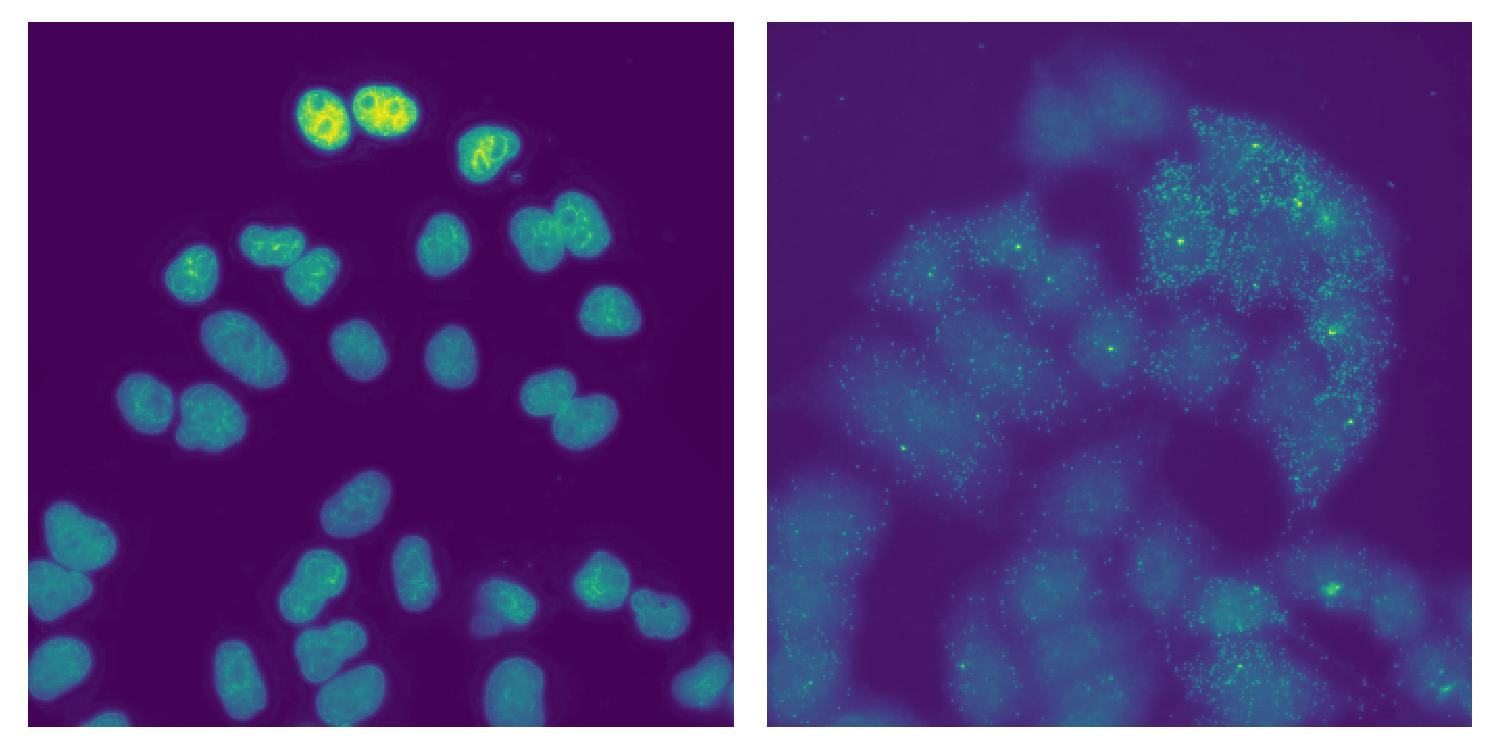
\includegraphics[width=\textwidth]{figures/chapter5/FoV_DYNLL2}
    \caption[Contrasted image with Dapi and smFISH channels]{Contrasted image with Dapi (\textit{left}) and smFISH (\textit{right}) channels.
	Images are projected in 2D.
	Targeted transcript is DYNLL2.
	Plot built with \emph{bigfish}}
    \label{fig:fov_racha}
\end{figure}

\subsubsection{Semi-automated RNA detection}

\ac{RNA} detection was performed with a Python implementation of FISH-quant v1~\cite{mueller_fish-quant_2013}.
In short, I applied a \ac{LoG} filter on the 3D \ac{smFISH} images, then a local maximum detection algorithm to localize individual RNA molecules.
This detection requires a manually set intensity threshold for every experiment to discriminate the actual RNAs from the noisy background.
Large agglomeration of spots were decomposed with a Gaussian mixture model, based on previous work~\cite{samacoits_computational_2018}.
Ultimately, \ac{RNA} foci were detected with the DBSCAN algorithm~\cite{ester_density-based_1996} applied on the detected spot positions: a foci is then defined as a set of at least 5 RNAs  with a maximum distance of 350 nanometers between RNAs belonging to the same foci.
Foci overlapping the nuclear area in the projected 2D images were considered as a transcription site and removed from the analysis.
Percentages of \ac{RNA} in foci were then calculated as number of \ac{RNA} inside the foci divided by the number of cytoplasmic \ac{RNA}s.

I would like to highlight two main differences compared to the current detection methods implemented in FISH-quant v2 (presented in Chapter~\ref{ch:chapter2}), both of which I improved: a detection threshold has to be set manually and the decomposition of agglomerated spots has since been simplified.

\subsubsection{Cell and nucleus segmentation}

Nuclear segmentation was performed from the DAPI channel and cellular segmentation from the cell autofluorescence in the \ac{smFISH} channel.
Segmentation was performed in 2D for both nuclei and cells, thus 3D images are projected in two dimensions using their maximal local focus values~\cite{tsanov_smifish_2016}.

Nuclei were segmented with NucleAIzer~\cite{hollandi_nucleaizer_2020}, a deep neural network pipeline trained with the annotations from the Data Science Bowl 2018 challenge\footnote{\url{https://www.kaggle.com/c/data-science-bowl-2018}}.
This pipeline is based on a Mask R-CNN architecture~\cite{He_2017_ICCV}, with optionally a fine-tuning of the segmented boundaries with a U-Net model~\cite{Ronneberger_2015}.
After a first round of segmentation, some nuclei were missing, so I removed the segmented nuclei from the DAPI channel and re-analyzed the image with the remaining nuclei again with NucleAIzer.
Removing the segmented nuclei from the original image implied the morphological reconstruction technique described in Chapter~\ref{ch:chapter3}.
This technique is now implemented in FISH-quant.

Cells were then segmented with a watershed algorithm using the nuclei masks as seeds.
A threshold value was set manually for every experiment to discriminate the cell surface from the background.
In case of poor results, some segmentation masks were corrected manually.
This was especially the case for transcripts that tend to localize in cell protrusions.
Further, accurate cellular segmentation is especially important for this localization pattern (also because only RNAs detections overlapping segmented cells are considered in our analysis).

\subsubsection{Localization feature engineering}

Based on the segmentation masks and the coordinates of the detected spots, I identified 9,710 individual cells with an average of 346 \ac{RNA}s per cell.
For each cell, I collected the cell and nucleus masks in 2D, the \ac{RNA} and the potential cluster coordinates in 3D.
In addition I saved an image of the cell, for visualization purposes, and different information about the experiment (the presence of a treatment, the targeted gene, etc.).
Cropped cells on the edge of the image and cells with less than 30 detected \ac{RNA} inside were removed.
At this point, I had a coordinate representation of every cell, as presented in Chapter~\ref{ch:chapter4}.

I designed and computed a set of 15 localization features to describe the spatial distribution of RNAs inside the cell:
\begin{itemize}
	\setlength\itemsep{0.1em}
	\item The number of foci.
	\item The proportion of \ac{RNA}s inside foci.
	\item The proportion of \ac{RNA}s inside the nucleus.
	\item The average \ac{RNA} distance to the cell membrane, normalized by the value obtained under a uniform \ac{RNA} distribution.
	\item The average \ac{RNA} distance to the nucleus membrane, normalized by the value obtained under a uniform \ac{RNA} distribution.
	\item The average foci distance to the cell membrane, normalized by the value obtained under a uniform foci distribution.
	\item The average foci distance to the nucleus membrane, normalized by the value obtained under a uniform foci distribution.
	\item The proportion of \ac{RNA}s inside cell protrusions.
	A protrusion region is defined by calculating the difference between the segmented cellular region and its morphological opening with a large window.
	\item The peripheral dispersion index, defined as the squared point distance to the centroid of the cell and normalized by the value obtained under a uniform \ac{RNA} distribution.
	\item The number of \ac{RNA}s within 515 nm from the nucleus membrane, normalized by the value obtained under a uniform \ac{RNA} distribution.
	\item The number of \ac{RNA}s between 515 nm and 1030 nm from the nucleus membrane, normalized by the value obtained under a uniform \ac{RNA} distribution.
	\item The number of \ac{RNA}s between 1030 nm and 1545 nm from the nucleus membrane, normalized by the value obtained under a uniform \ac{RNA} distribution.
	\item The number of \ac{RNA}s between 0 nm and 515 nm from the cell membrane, normalized by the value obtained under a uniform \ac{RNA} distribution.
	\item The number of \ac{RNA}s between 515 nm and 1030 nm from the cell membrane, normalized by the value obtained under a uniform \ac{RNA} distribution.
	\item The number of \ac{RNA}s between 1030 nm and 1545 nm from the cell membrane, normalized by the value obtained under a uniform \ac{RNA} distribution.
\end{itemize}

The size of the concentric regions for the last 6 features were determined to be 5 pixels based on visual inspection of the samples.
A conversion to nanometer (with a pixel-size of 103nm) results in the reported ranges.

\subsubsection{Binary classification models}

\begin{figure}[]
	\centering
	\minipage{0.2\textwidth}
		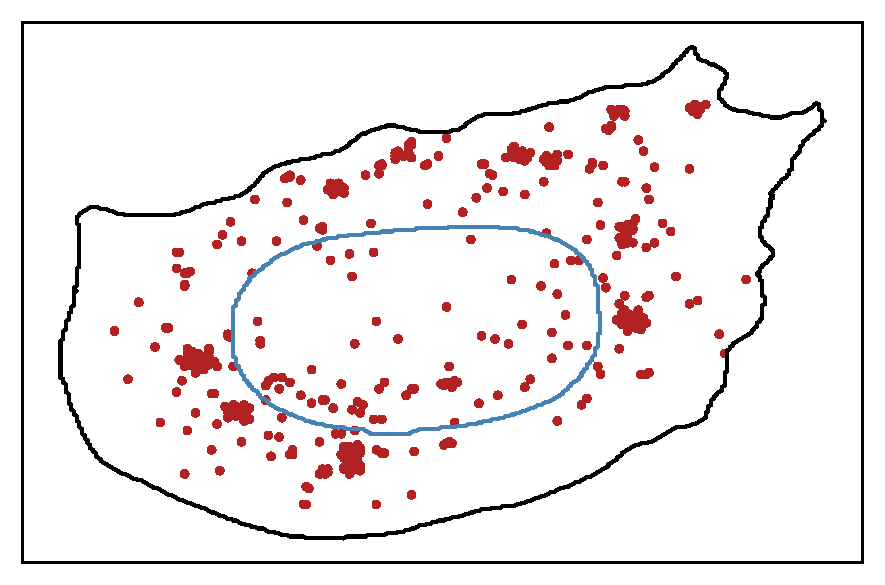
\includegraphics[trim={0.5cm 0.5cm 0.5cm 0.5cm},clip,width=\linewidth]{figures/chapter5/plot_foci}
		\subcaption{Foci}
	\endminipage\hfill
	\minipage{0.2\textwidth}
		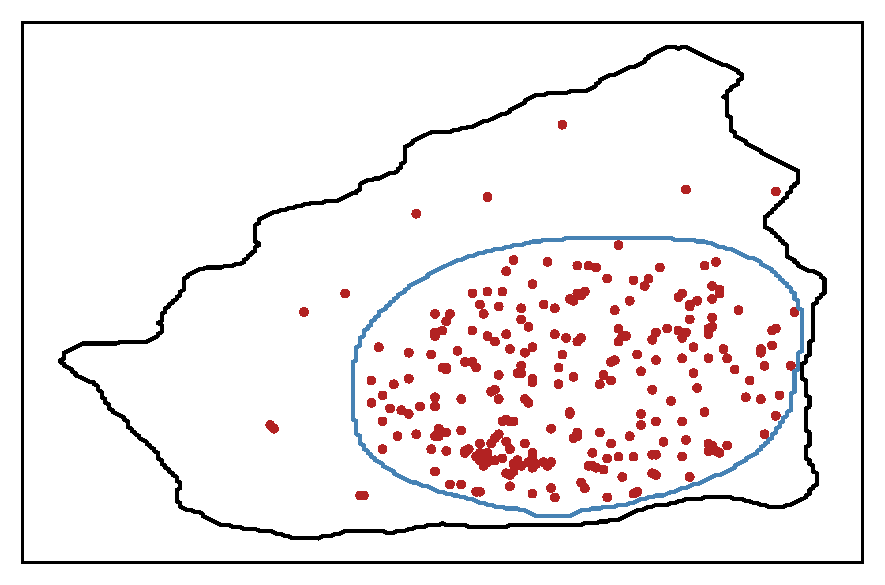
\includegraphics[trim={0.5cm 0.5cm 0.5cm 0.5cm},clip,width=\linewidth]{figures/chapter5/plot_intranuclear}
		\subcaption{Intranuclear}
	\endminipage\hfill
	\minipage{0.2\textwidth}
		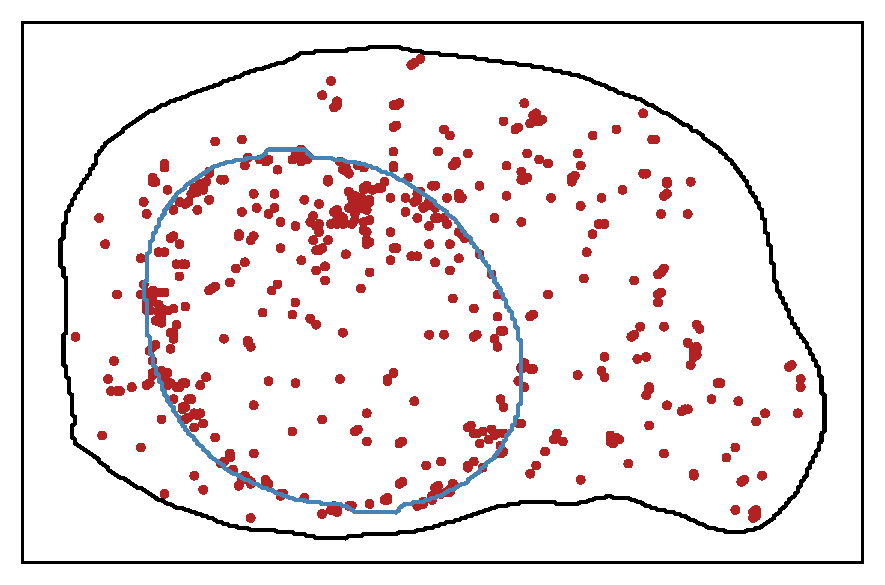
\includegraphics[trim={0.5cm 0.5cm 0.5cm 0.5cm},clip,width=\linewidth]{figures/chapter5/plot_nuclear}
		\subcaption{Nuclear edge}
	\endminipage\hfill
	\minipage{0.2\textwidth}
		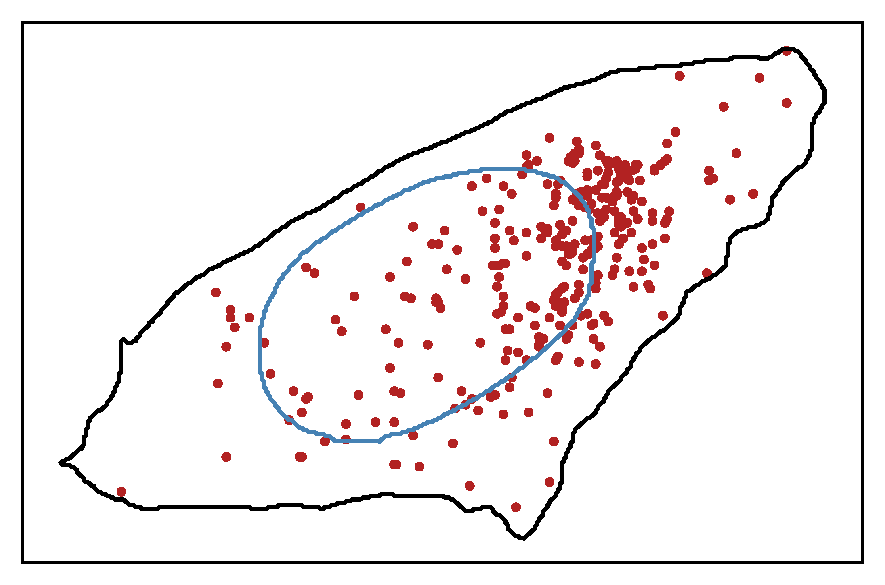
\includegraphics[trim={0.5cm 0.5cm 0.5cm 0.5cm},clip,width=\linewidth]{figures/chapter5/plot_perinuclear}
		\subcaption{Perinuclear}
	\endminipage\hfill
	\minipage{0.2\textwidth}
		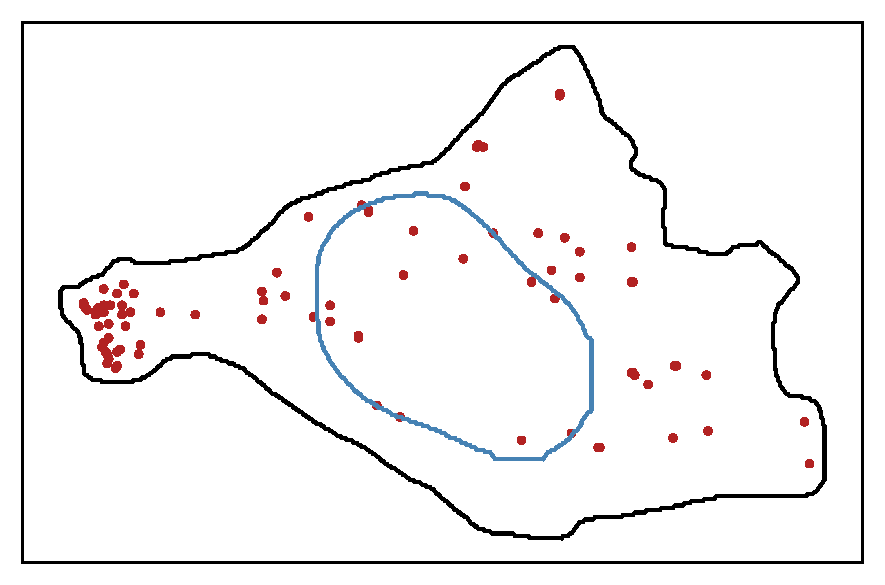
\includegraphics[trim={0.5cm 0.5cm 0.5cm 0.5cm},clip,width=\linewidth]{figures/chapter5/plot_protrusion}
		\subcaption{Protrusion}
	\endminipage
	\caption[RNA localization patterns]{RNA localization patterns from~\cite{CHOUAIB_2020}.
	Coordinate representations with RNA spots (\textit{red}), cell membrane (\textit{black}) and nuclear membrane (\textit{blue}).
	Detection and segmentation results are extracted and visualized with \emph{bigfish}}
	\label{fig:localization_patterns_racha_features}
\end{figure}

I used these hand-crafted features to train several binary classifiers, one for each localization pattern we wanted to recognize: foci, intranuclear, nuclear edge, perinuclear, protrusion.
Random localization was considered by default.
Figure~\ref{fig:localization_patterns_racha_features} illustrates an example of these patterns with a coordinate representation.

To train the classifiers, manual annotations were needed as a ground truth.
I generated panels with the cropped original image of the individual cells and their coordinate representations.
These panels were then manually tagged with the appropriate localization pattern by several experienced microscopists.
This resulted in a dataset of 810 annotated cells (Table~\ref{table:real_dataset_chapter5}).

\begin{wraptable}{L}{0.50\textwidth}
	\centering
	\begin{tabular}{| c | c |}
		\hline
		Pattern & \# of cells \\
		\hline
		Random & 372\\
		Foci & 198\\
		Intranuclear & 73\\
		Nuclear edge & 87\\
		Perinuclear & 64\\
		Protrusion & 83\\
		\hline
	\end{tabular}
	\caption[Count of annotated cells]{Annotated cells}
	\label{table:real_dataset_chapter5}
\end{wraptable}

A first evaluation of how well our localization features describe the different localization classes was the visualization of the feature space.
To do so, I reduced the dimensionality with a \ac{t-SNE} transformation~\cite{vandermaaten_2008} in order to visualize the features point cloud.
I initialized the \ac{t-SNE} with a PCA transformation and used a perplexity value of 30.
From the original 15-dimensional feature space, I thus obtained a 2D vector representation that could be easily inspected.

I also defined a supervised learning problem with the training of 5 independent binary Random Forest classifiers~\cite{breiman_random_2001}.
Such a random forest classifier is an ensemble model of tree classifiers.
Each tree is trained on a subsample of the observations and a subset of features.
This ensembling framework makes random forest quite robust to overfitting.
The choice to design the problem as several binary classifiers instead of one multi-class problem allowed me to define the localization patterns as non mutually exclusives.
Indeed, an individual cell can display several patterns at the same time, like \ac{RNA} clusters (foci) localizing around the nuclear membrane (nuclear edge).
For each model, I then built a training set including all the cells of one class and a subsampling of cells from others classes, such that the imbalance is 1:4 for the positive class.
This is a so called ''one vs.\ all'' training strategy.
For every sample, an \ac{OOB} prediction can be computed using only the trees fitted without the sample.
In such manner, the model can ''be fit in one sequence, with cross-validation being performed along the way.''~\cite{hastie_elements_2009}.
I initialized the random forests with 100 trees, a maximal depth of 3 and a minimum number of samples per splitter node of 2.
During the training, for each split, I considered a subset of 10 features and entropy criterion.
In addition, input dataset was rescaled to have zero mean and unit variance.

\subsection{Results}
\label{subsec:results_general_pattern}

It is widely known that RNAs levels of a given gene can vary substantially from one cell to another.
Thanks to their design and/or their normalization, our spatial features are mostly invariant to \ac{RNA} concentration.
They enable the use of unsupervised or supervised methods to classify cells among several localization patterns without the compounding impact of gene expression variability.

\subsubsection{Unsupervised visualization}

\begin{figure}[]
    \centering
    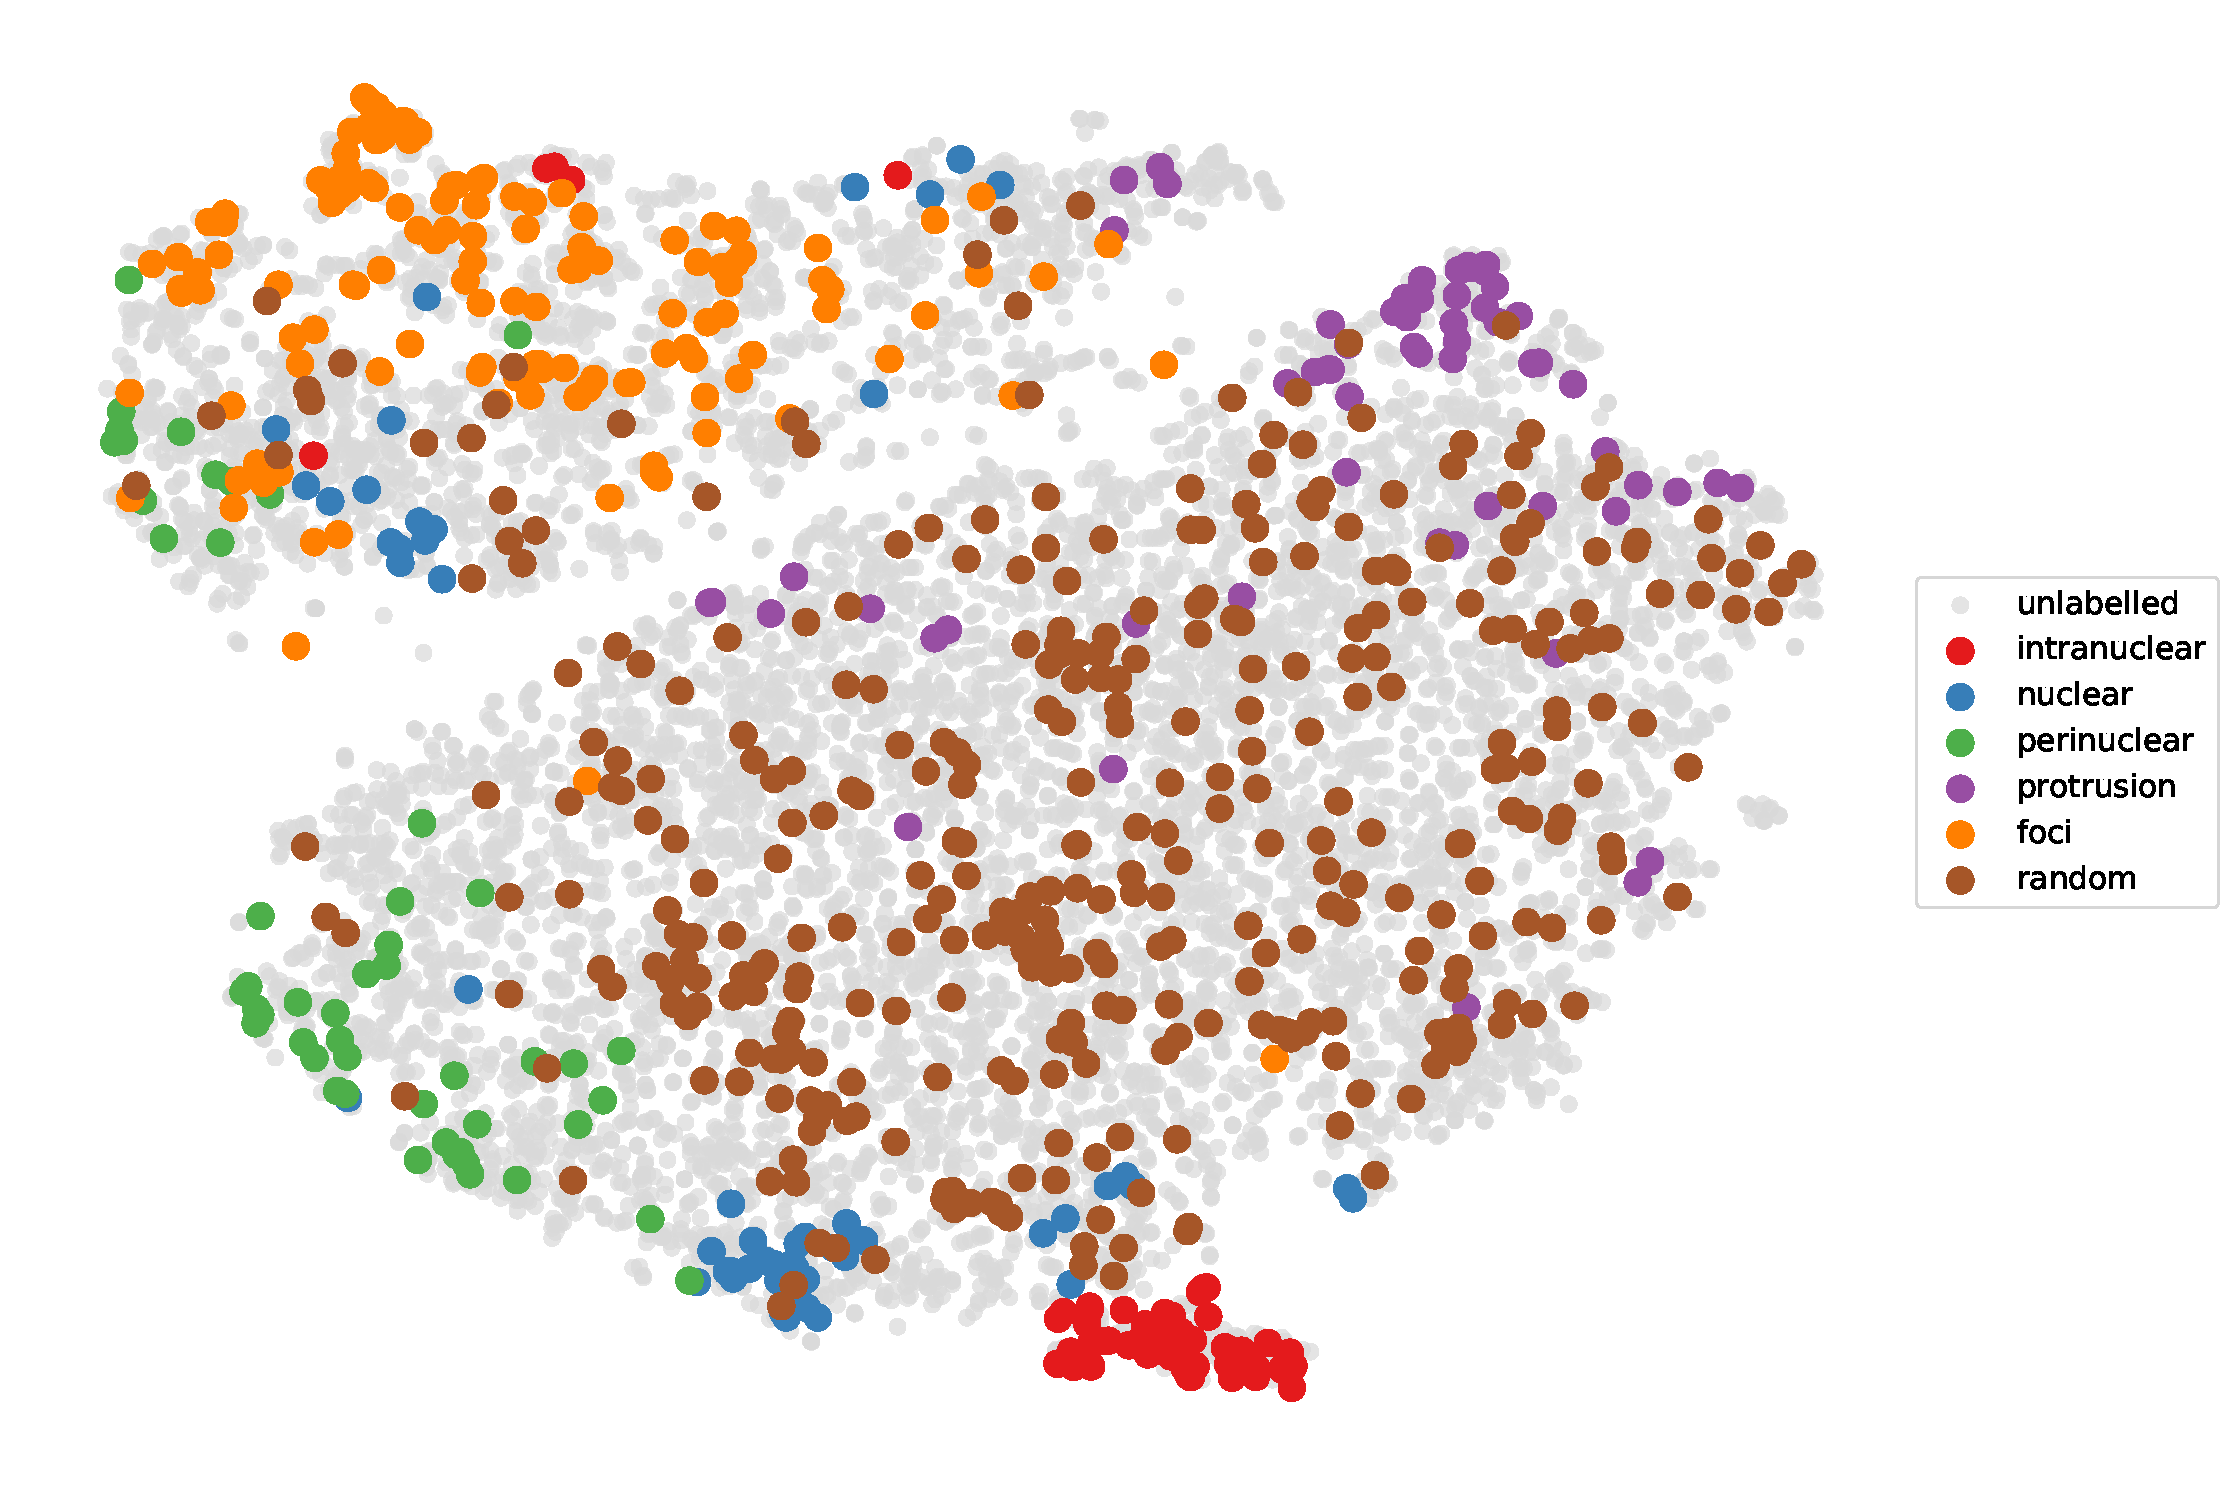
\includegraphics[width=\textwidth]{figures/chapter5/tsne_annotation_legend}
    \caption[t-SNE embedding of experimental cells]{t-SNE embedding from~\cite{CHOUAIB_2020}.
	Each point is a cell in the feature space after a t-SNE transformation.
	Manually annotated cells are colored according to their localization pattern.
	Cells that were not annotated or that had multiple patterns are colored in gray}
    \label{fig:tsne_annotation_racha}
\end{figure}

The resulting embedding from the \ac{t-SNE} algorithm can be observed in Figure~\ref{fig:tsne_annotation_racha}.
Cells with different patterns are localized in different regions of the embedded feature space.
Moreover, cells with the same annotations, cluster in the same regions independently of their targeted gene.
This suggests that the hand-crafted features capture key information of the localization patterns.

Initializing the \ac{t-SNE} algorithm with a PCA transformation results in a better preservation of the global data structure, thus enabling more relevant global interpretation.
In particular, we can discriminate at the top a large cluster of cells with a foci pattern from the rest of the cell population.
The resulting embedding also seems to polarize between nucleus-related patterns (bottom left) and the cell-related patterns (top right).
This polarization remains even among the subpopulation with potential foci pattern.

Such conclusion validates the design to let a cell being classified with several non-exclusive localization patterns.
Indeed, a foci can be localized in one of several relevant subcellular compartments.

\subsubsection{Supervised classification}

The result presented above showed that the feature space discriminates well between localization classes.
Next, I wanted to test how well these features perform when used in a random forest classifier.

For this, I computed 5 binary predictions, one per pattern, for each cell.
A pattern was then assigned to a cell if the probability given by the random forest classifier for that pattern was higher than 0.5.
If no pattern was detected, the cell was classified with a random localization pattern.
In total, I analyzed 27 different genes in a total of 9,710 cells.

The \ac{OOB} accuracy score obtained for the different patterns was between 0.93 and 0.99, while a dummy classifier only returned a 0.8 accuracy score (the dataset was built with 20\% positive samples).
Among all patterns, intranuclear localization was the easiest to detect.
On the other hand, the nuclear edge and perinuclear patterns were the most difficult to classify due to possible confusion with a random pattern or the lack of annotated cells.

The total number of cells per gene varied, thus predictions were aggregated for each gene.
This aggregation also facilitated data inspection and a first comparison among genes.
For every gene, I computed the proportion of cells displaying each indicated localization pattern.
Results were eventually reported in a heat map~\ref{fig:heatmap_racha}, for every gene and pattern.
Importantly, row values did not sum to one because classifiers (and so columns predictions) were independent.

\begin{wraptable}{R}{0.50\textwidth}
	\centering
	\begin{tabular}{| c | c |}
		\hline
		Pattern & Accuracy score\\
		\hline
		Random & -\\
		Foci & 0.95\\
		Intranuclear & 0.99\\
		Nuclear edge & 0.93\\
		Perinuclear & 0.93\\
		Protrusion & 0.94\\
		\hline
		\textit{Dummy classifier} & \textit{0.80}\\
		\hline
	\end{tabular}
	\caption[Random forest accuracy]{Random forest accuracy (OOB)}
	\label{table:accuracy_oob}
\end{wraptable}

We manually identified a group of random genes that could be used as a control group: KIF20B, MYO18A, SYNE2 and PLEC.
This control group permitted to perform statistical testing over the aggregated predictions.
A Fisher's exact test can measure if the proportion of cells observed with a pattern is significantly greater than the proportion observed in the control group (with a $\text{p-value} < 10^{-3}$).
Genes whose transcripts presented a significant localization preference are reported in Figure~\ref{fig:heatmap_racha}.

\begin{figure}[]
    \centering
    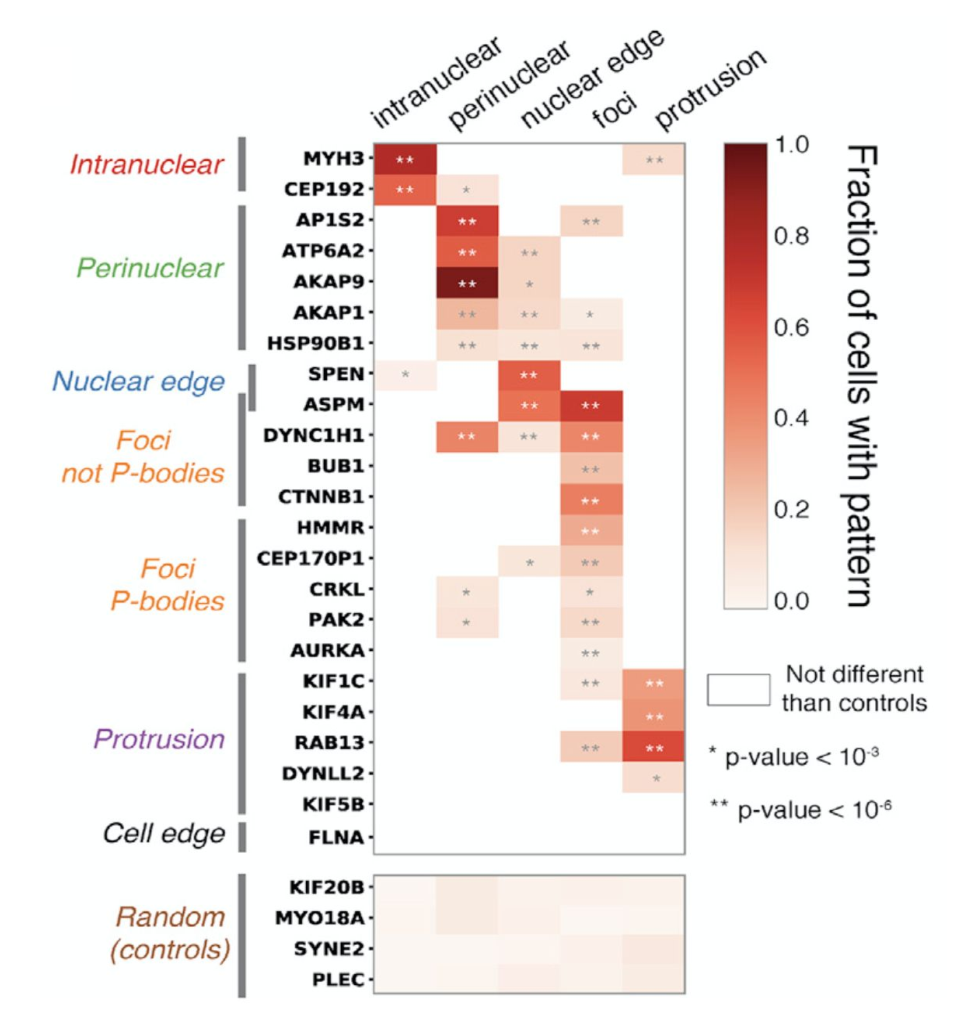
\includegraphics[width=\textwidth]{figures/chapter5/heatmap_racha_2}
    \caption[Heat maps with localization pattern classification results]{Heat maps from~\cite{CHOUAIB_2020} with the fraction of cells classified in the indicated pattern.
	(\textit{Top heat map}) Genes whose RNAs shows a localization preference.
	Only values significantly different from negative controls are colored (p-value computed with Fisher's exact test).
	(\textit{Bottom heat map}) Negative control with genes whose RNAs localize randomly.
	(\textit{Left bars}) Manual annotations of the genes are indicated with the same color scheme than Figure~\ref{fig:tsne_annotation_racha}}
    \label{fig:heatmap_racha}
\end{figure}

Overall, we observed consistent results between the automated analysis and the manual annotations performed by the biologists (the colored annotations in the \ac{t-SNE} plot~\ref{fig:tsne_annotation_racha} and the vertical colored bars next to the heat map~\ref{fig:heatmap_racha}).
The agreement between automated and manual classification held with a high degree of statistical significance, except for FLNA and KIF5B.
More specifically, FLNA transcripts were manually annotated with a potential cell edge pattern.
However, this localization pattern was difficult to recognize with the quantitative pipeline, mostly because the pattern is only visible in 3D while the cell segmentation, and the spatial features resulting from it, was in 2D.
For these reasons we did not study in depth this localization pattern.

\subsubsection{Recognition of five localization patterns}

Apart from KIF5B, others transcripts localizing in cellular  protrusions were correctly identified: KIF1C, KIF4A, RAB13 and DYNLL2.
The frequency of this pattern varied substantially, between 14\% and 62\% of cells classified, respectively for DYNLL2 and RAB13.
Interestingly, this pattern concerns four \ac{RNA}s encoding motor proteins: the three kinesins KIF1C, KIF4A, KIF5B and DYNLL2.

MYH3, another transcript encoding a motor protein, localized partially in protrusions, although it is not its most frequent localization pattern.
Most of the time, MYH3 transcripts remained in the nucleus, exhibiting an intranuclear pattern.
This is the most easily recognizable pattern: more than 55\% of cells spotting MYH3 and CEP192 \ac{RNA}s showed an accumulation of transcripts inside nucleus.

The two genes observed with a nuclear edge pattern, ASPM and SPEN, had 50\% and 55\% of cells identified with this localization, respectively.

Several genes were identified with \ac{RNA}s in the perinuclear area: AKAP1, AKAP9, AP1S2, ATP6A2, and HSP90B1.
The number of cells displaying this pattern ranged from 13\% (HSP90B1) to 93\% (AKAP9).
Even with a small number of cells, HSP90B1 showed a significant perinuclear pattern compared to the control group.
In our study, we could then further show that HSP90B1 localizes to the the endoplasmic reticulum, and that this localization is translation dependent.

A large number of transcripts were found to localize in foci.
We classified them in two groups, with a more detailed analysis in the Section~\ref{sec:translation_factories}.
The first group contains transcripts accumulating in \ac{P-bodies}: AURKA, HMMR, CEP170P1, CRKL and PAK2.
The second group includes ASPM, DYNC1H1, BUB1 and CTNNB1 transcripts, accumulating in non-\ac{P-bodies} foci we call translation factories.
It is noteworthy to mention that a number of genes exhibited foci with another localization preference in parallel like ASPM (nuclear edge), DYNC1H1, AP1S2, AKAP1, HSP90B1 (perinuclear), KIF1C and RAB13 (protrusion).
In general, non-\ac{P-bodies} genes had a higher proportion of cells classified with a foci pattern: between 24\% (BUB1) and 69\% (ASPM) cells while \ac{P-bodies} genes have between 7\% (AURKA) and 31\% (HMMR) cells.
Likewise, in term of RNA content, non-\ac{P-bodies} genes had a higher proportion of \ac{mRNA} in foci, varying from 9\% (BUB1) to 28\% (CTNNB1), while \ac{P-bodies} accumulated between 2\% to 15\% of \ac{mRNA}s.
This foci quantification is in line with the previously reported estimations in the literature of 10\% to 20\% \ac{mRNA}s clustered in foci~\cite{Pillai_2005, Hubstenberger_2017}.

\subsubsection{Cell-to-cell variability}

We then focused on individual cells instead of the aggregated information per gene.
This showed a remarkable heterogeneity of \ac{RNA} localization.
For example, for CTNNB1, we observed a binary behavior, with cells either having no foci at all or alternatively more than 60\% of \ac{mRNA}s clustered in foci.

For a more detailed quantification of this intercellular variability, I would like to refer the reader to Appendix~\ref{ch:cell_pattern_classification}.
Cells of specific genes are plotted on \ac{t-SNE}~\ref{fig:tsne_proba_gene} and single cell results are summarized in heat maps~\ref{fig:heatmap_racha_cells}.
Pattern probabilities returned by classification models varied from cell to cell.
For a given gene, cells were dispersed on the \ac{t-SNE} plot, although a majority of them still accumulated in the expected area.
Finally, some cells had simultaneously several localization patterns.
As mentioned above, this is frequently the case with cells having \ac{RNA} foci, where foci can be either found in protrusion or close to the nucleus.
Likewise, MYH3 cells frequently showed an intranuclear and protrusion pattern.

In conclusion, my quantitative pipeline confirmed the manual observations and measured a high degree of heterogeneity of \ac{RNA} localization across individual cells.
This variability is a general phenomenon, at least for HeLa cells, since it is seen with nearly all the genes analyzed in~\cite{CHOUAIB_2020}.

\section{Local translation and translation factories}
\label{sec:translation_factories}

Beyond the generic pattern recognition pipeline I have implemented, another important quantitative result is related to \ac{RNA} and their implication in translation, a phenomenon we termed \emph{translation factory}.
This analysis is part of a broader investigation about the co-localization of \ac{mRNA}s and their encoded proteins, a major contribution of~\cite{CHOUAIB_2020}

\subsection{Introduction}
\label{subsec:introduction_translation_factories}

In contrast to previous studies on \ac{RNA} localization~\cite{lecuyer_global_2007, battich_image-based_2013, Chen_2015, eng_seqfish_2019, Xia_2019}, our experimental design also permitted to detect translated proteins.
In brief, we used a library of HeLa cell lines, were in each cell line a \ac{BAC} including a \ac{GFP}-tagged gene~\cite{poser_bac_2008} was introduced.
This allows not only to visualize the RNA with FISH probes again the GFP signal, as exploited above in the study of RNA localization, but also to visualize the translated protein in the GFP channel.
In~\cite{CHOUAIB_2020}, we performed a high-content screen in HeLa cells and visualize simultaneously the \ac{mRNA} and its encoded protein.

Along with \ac{RNA} localization patterns, we observe occurrences of local translation in several subcellular areas.
For example, the phenomenon is observed in the nuclear membrane with the ASPM and SPEN transcripts.
Some local translations are expected, like HSP90B1 (an endoplasmic reticulum protein), ATP6A2 (in endolysosomes) or AKAP1 (an \ac{RBP} at the surface of mitochondria).
Others are discoveries like AKAP9 or AP1S2, whose \ac{mRNA}s are known to localized respectively in the Golgi or on endosomes.

Our collaborators further used the SunTag system, which allows to visualize the presence of nascence peptide chains, and hence ongoing translation~\cite{pichon_visualization_2016, Pichon_2018, Wu_2016}.
While this required genetic engineering, to include the SunTag sequence into the gene of interest, it provides important information about co-translational targeting.
Here, this technique allows us to confirm that both ASPM \ac{mRNA}s and nascent proteins localized in nuclear membrane, thus suggesting a local translation.

The remainder of this section will detail our analysis of the translation-dependent foci pattern.
When investigating the \ac{RNA}s that form foci, we found that most co-localize with P-body markers.
Such localization in P-bodies has been linked to RNA storage or degradation.
In contrast, we found four transcripts that accumulate in foci, but do not colocalized with P-body markers: BUB1, DYNC1H1, CTNNB1 and ASPM.
Interestingly, we found that these foci disappear when cells were treated with a translation inhibitor.
Further analysis revealed a co-localization of RNA foci and nascent proteins~\ref{fig:translation_factory}.
Taken together, this suggests that these foci bring together RNAs, which are locally translated.
We hence named these complexes \emph{translation factories}, where specific \ac{mRNA}s accumulate to be translated, and not repressed.
My second contribution to~\cite{CHOUAIB_2020} was the quantification of this unexpected phenomenon, exploiting my cluster detection methods and experiments with a translation inhibition protocol.

\begin{figure}[]
    \centering
    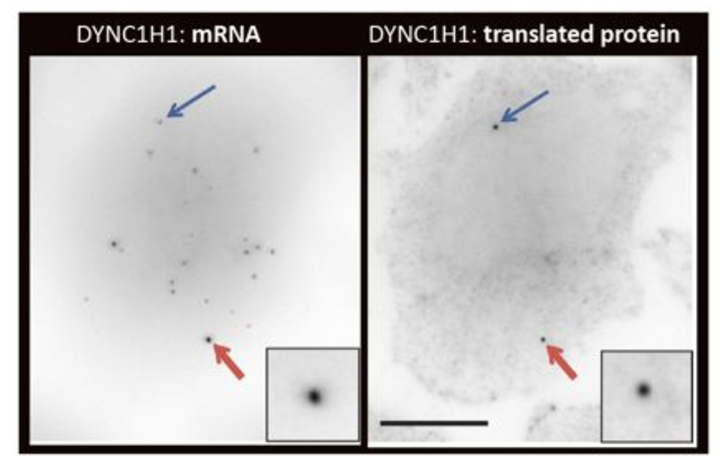
\includegraphics[width=\textwidth]{figures/chapter5/translation_factory}
    \caption[smFISH and SunTag images of DYNC1H1]{Colocalization between the DYNC1H1 transcript and its nascent protein, from~\cite{pichon_visualization_2016}.
	Transcripts and proteins are targeted with smFISH probes (\textit{Left}) and SunTag (\textit{Right}) respectively.
	\textit{Scale bar} is 10$\mu$m}
    \label{fig:translation_factory}
\end{figure}

\subsection{Materials and methods}
\label{subsec:materials_translation_factories}

In the continuation of the work presented in Section~\ref{sec:general_pattern_recognition}, the quantification was developed in Python and available online\footnote{\url{https://github.com/Henley13/paper_translation_factories_2020}}.

\subsubsection{Translation inhibition}

To analyze the role of translation in \ac{mRNA} localization, we performed several experiments where translation is inhibited by either Puromycin or Cycloheximide.
Coupled with my computational pipeline, we could then measure the impact of a translation inhibition.

While both drugs inhibit translation, they differ in the their mode of action:
Puromycin inhibits translation by releasing the nascent peptide chain from the ribosomes, while Cycloheximide freezes the ribosomes on the \ac{mRNA}s.
Importantly, the latter results in the nascent peptide chain still being present at the translated RNA.
If RNA localization patterns are impacted by these drug treatments, this localization is likely driven by translation.
Furthermore, these two treatments allow to clarify if a translation-dependent localization requires the nascent peptide chain.
In the case of ASPM gene, we observed for example that the localization patterns (nuclear edge and foci) disappeared with Puromycin, but not with Cycloheximide.
It suggests that the \ac{mRNA} localization requires the nascent protein.

\subsubsection{Foci detection}

Both on the treated and untreated cells, I applied my spot detection algorithms, the decomposition algorithm for RNA aggregates, and finally the \ac{RNA} cluster detection (see Subsection~\ref{subsec:materials_general_pattern}).
It is important to note that the cluster detection is distinct from the decomposition of dense areas.
Such areas can indeed be processed in a way that no cluster is detected afterward.

\subsection{Results}
\label{subsec:results_translation_factories}

\subsubsection{Translation-dependent localization}

\begin{figure}[]
    \centering
    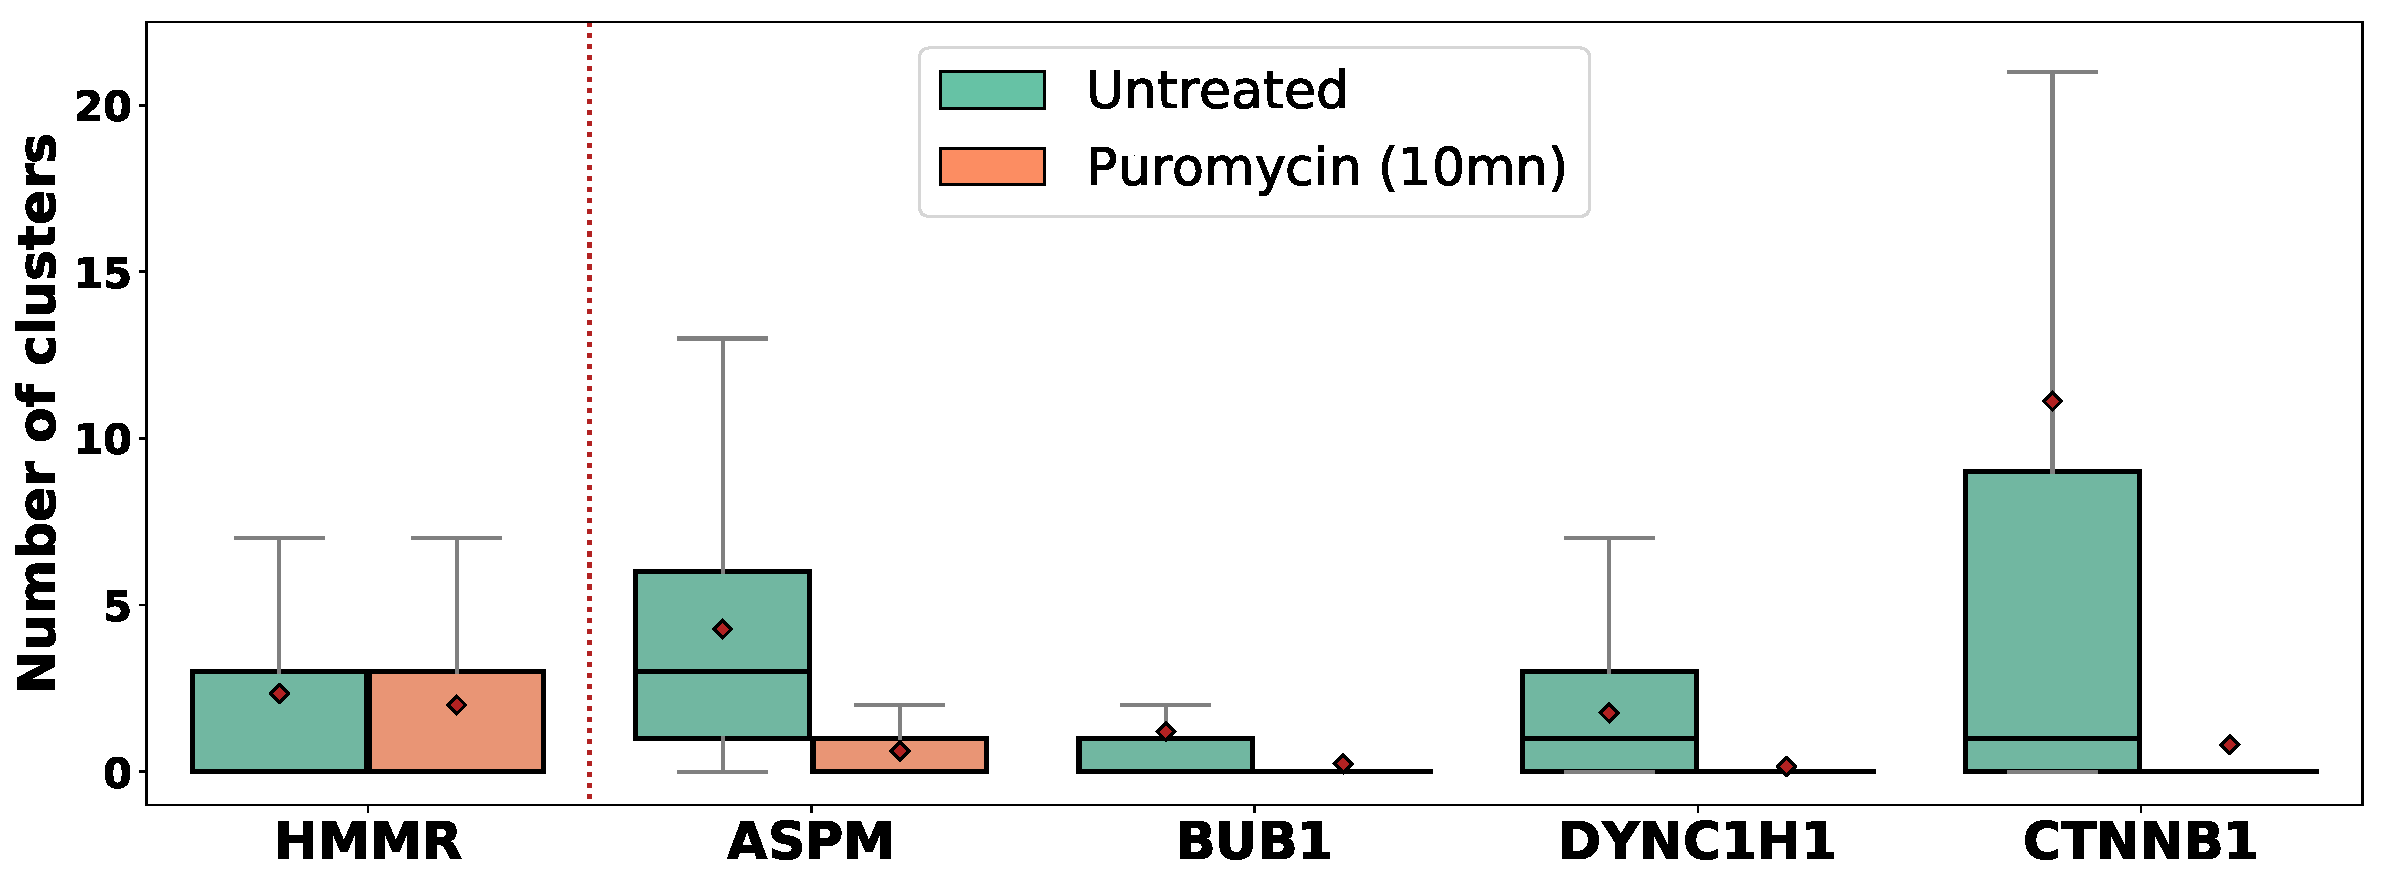
\includegraphics[width=\textwidth]{figures/chapter5/plot_puromycin}
    \caption[Box plot with the number of detected RNA foci]{Box plot with the number of detected RNA foci for different genes and treatments.
	Red diamonds are the mean and the \textit{whiskers} equal 1.5 the interquartile range}
    \label{fig:plot_puromycin}
\end{figure}

An obvious indicator to assess if a foci pattern is disrupted is the number of \ac{RNA} foci detected per cell.
When I compared treated and untreated cells, the difference is clear for the four genes BUB1, DYNC1H1, CTNNB1 and ASPM.
Their transcripts usually accumulate in foci, but with the presence of Puromycin, \ac{mRNA}s are dispersed within the cell and the number of detected foci drops.
An analysis with a finer granularity is detailed in Appendix~\ref{ch:cell_pattern_classification} and especially in Figure~\ref{fig:tsne_proba_gene}, where changes on the single cell level are reported.
In addition, a dual-color \ac{smiFISH} allowed us to visualize two different transcripts at the same time and showed that the foci detected for these four genes are not overlapping.
These are hence distinct \ac{RNA} complexes.

As a comparison, in Figure~\ref{fig:plot_puromycin}, I performed the same analysis with HMMR, a gene found in \ac{P-bodies}.
The difference is striking, as the foci pattern seems unchanged when translation is inhibited.

Taken together, this leads us to the conclusion that for these four genes, the RNA foci are acting as translation factories.

\subsubsection{CTNNB1: translation and degradation}

Among the four genes with translation factories, cytoplasmic foci of CTNNB1 \ac{mRNA} present a surprising regulation mechanism.
This \ac{mRNA} encodes the $\beta$-catenin protein, which is the main transcription factor of the Wnt signaling pathway~\cite{Grainger_2018}.
The later is known to play a role in carcinogenesis and embryogenesis.
The Wnt signal allows the $\beta$-catenin protein to translocate and accumulate in the nucleus in order to activate targeted transcriptions.

The existence of translation factories offers a new insight on the dynamic at stakes in the presence of Wnt.
$\beta$-catenin is degraded in a ''destruction complex'' that involves APC, AXIN, in addition to the kinases CK1$\alpha$ and GSK3~\cite{stamos_catenin_2013}.
When the Wnt pathway is activated, these molecules are recruited to the cell membrane and can no longer interact with $\beta$-catenin, thus stopping its degradation.
As a consequence, we observed that $\beta$-catenin is highly expressed and accumulates in the nucleus.
Interestingly, in the presence of Wnt, we also observed that the CTNNB1 \ac{mRNA} foci disappear.
This phenomenon suggests a relation between the degradation of $\beta$-catenin and foci formation.
In~\cite{CHOUAIB_2020} we demonstrated that CTNNB1 translation factories rely on the nascent peptide chain, but it seems they also require the ''destruction complex''.
When the different components of this complex are disrupted, the \ac{mRNA} foci tend to disappear.
Moreover, these components accumulate in the foci.
CTNNB1 translation factories are thus sites of both $\beta$-catenin synthesis and degradation.
As~\cite{Chin_2020} summarizes it, these factories are ''sites of co-translational protein degradation, where CTNNB1 protein rapidly comes into contact with the destruction complex, offering an elegant mechanism to tightly control the cellular levels of potent signaling pathway effectors''.

\section{A translation and cell cycle dependent centrosomal pattern}
\label{sec:centrosomal}

For the analysis in~\cite{safieddine_choreography_2021} I could further validate and refine my analysis pipeline, and already automated workflows permitted a substantially faster analysis.
Specifically, it benefits from the development of FISH-quant v2 and the improvements published in the literature about cell segmentation~\cite{Imbert_fq_2022, stringer_cellpose_2021}.
My contribution to this study was the quantification of the centrosomal localization pattern observed for some \ac{mRNA}s.

\subsection{Introduction}
\label{subsec:introduction_centrosomal}

This study is a follow-up of the above described screen, with the goal to link RNA localization and translation at centrosomes.

Centrosomes have an important role in cell division, in addition to regulate cell motility and polarity~\cite{wu_2017}.
Before cell division, the centrosome duplicates.
As soon as division begins, the two centrosomes move to opposite ends of the cell.
Microtubules then assemble into a spindle between the two centrosomes, which then helps to separate the replicated chromosomes into the two daughter cells.

First observations of a \ac{mRNA} accumulation at the centrosomes were made on Xenopus early embryos~\cite{Groisman_2000}, with cyclin B1 \ac{mRNA}s concentrating at the mitotic apparatus.
Subsequent approaches of microscopy with \ac{FISH} techniques allow to image \ac{mRNA} localization in Drosophila~\cite{lecuyer_global_2007, wilk_diverse_2016} and human cell lines~\cite{Sepulveda_2018, CHOUAIB_2020}.
As these \ac{mRNA}s encode for known centrosomal proteins, these studies suggest a phenomenon of local translation.

In~\cite{safieddine_choreography_2021}, we identified 8 \ac{mRNA}s with a centrosomal pattern.
Remarkably, these \ac{mRNA}s displayed a RNA localization pattern with a dependence on the cell cycle.
Their localization appear to be translation dependent, through the synthesis of a nascent protein, and cell cycle dependent.
Moreover, these \ac{mRNA}s conserved their properties in both human and drosophila cell lines.

\subsection{Materials and methods}
\label{subsec:materials_centrosomal}

The quantitative analysis presented here exploits an improved version of \emph{bigfish}, especially for the spot detection.
This work was developed in Python and the code repository is public\footnote{\url{https://github.com/Henley13/paper_centrosome_2020}}.

\subsubsection{Experimental data}

Image acquisition was performed on an Opera Phenix High-Content Screening System (PerkinElmer).
We acquire 3D images with around 35 z-slices and a z-spacing of 0.3$\mu$m.
In total, and after curation, we collected 3,678 \ac{FoV}s of HeLa cell line for 12 different transcripts, with control experiments based on treatment with translation inhibitors Puromycin or Cycloheximide.
In addition to the \ac{smFISH} channel, each image stack includes three fluorescent labels to visualize the nucleus (DAPI), the cell (CellMask\textsuperscript{\texttrademark}) and the centrosomes (Centrin1-\ac{GFP}) as illustrated in Figure~\ref{fig:fov_adham}.

\begin{figure}[]
    \centering
    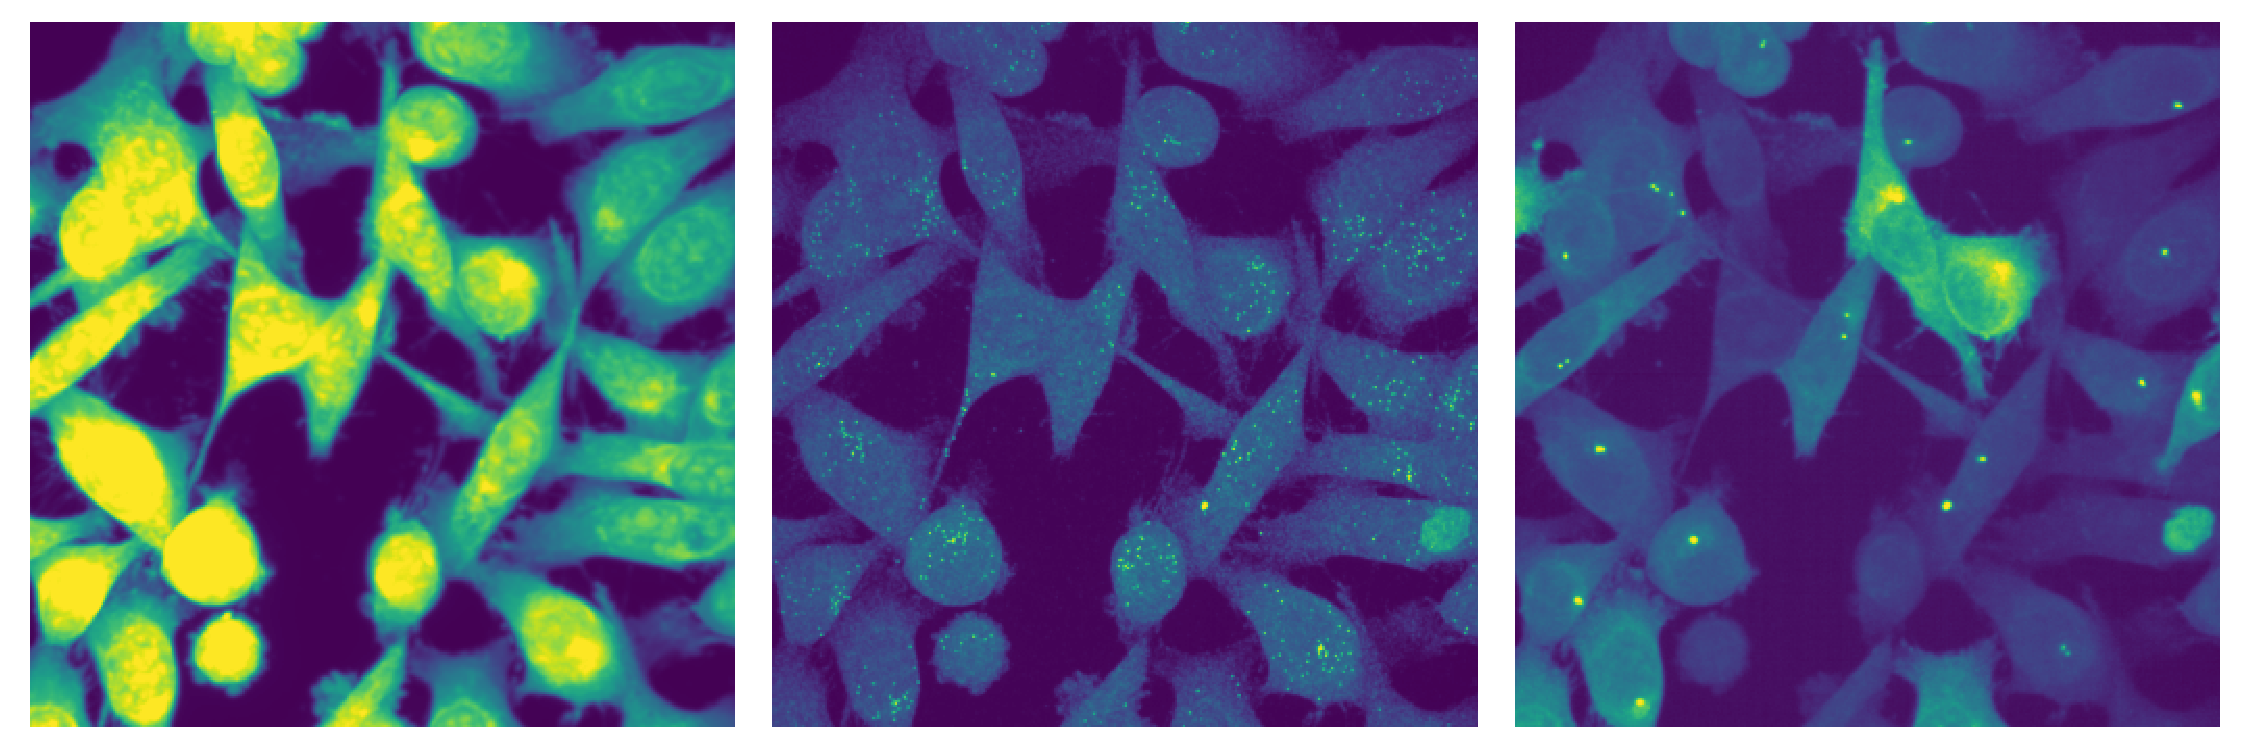
\includegraphics[width=\textwidth]{figures/chapter5/FoV_BICD2}
    \caption[Contrasted image with CellMask\textsuperscript{\texttrademark}, smFISH and GFP channels]{Contrasted image with CellMask\textsuperscript{\texttrademark} (\textit{left}), smFISH (\textit{center}) and GFP (\textit{right}) channels.
	Targeted transcript is BICD2.
	Images are projected in 2D.
	Plot built with \emph{bigfish}}
    \label{fig:fov_adham}
\end{figure}

\subsubsection{RNA and centrosome detection}

In~\cite{safieddine_choreography_2021}, and for the first time, I used the threshold-free spot detection described in Chapter~\ref{ch:chapter2}.
This heuristic approach permitted me to automatically detect RNA in thousands of images.
\ac{RNA} detection was followed by the decomposition of dense areas and the detection of \ac{RNA} foci, everything being processed from the \ac{smFISH} channel projected in 2D.

The novelty in this paper is the detection of centrosomes from a \ac{GFP} channel (projected in 2D).
Since the centrosome appears as a much larger spot than the individual \ac{RNA} molecule, I applied my \ac{RNA} cluster detection method with fine-tuned parameters.
This worked robustly, and allowed for an automated centrosome detection (Figure~\ref{fig:centrosomes}).

\begin{figure}[]
    \centering
    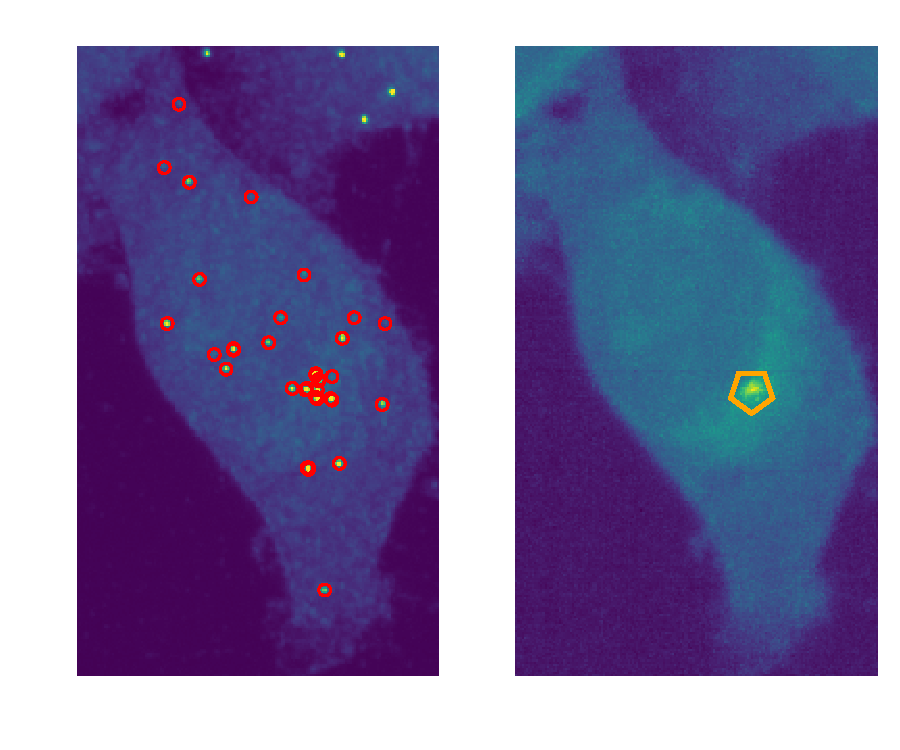
\includegraphics[width=\textwidth]{figures/chapter5/centrosomes}
    \caption[RNA and centrosome detection results]{Contrasted image with detected RNAs on a smFISH channel (\textit{left}) and detected centrosome on a GFP channel (\textit{right}).
	Targeted transcript is BICD2.
	Plot built with \emph{bigfish}}
    \label{fig:centrosomes}
\end{figure}

\subsubsection{Cell and nucleus segmentation}

Nucleus and cell segmentation was performed with a pretrained Cellpose model~\cite{stringer_cellpose_2021} from the 2D DAPI and CellMask\textsuperscript{\texttrademark} channels, respectively .
CellPose is based on a modified U-Net architecture~\cite{Ronneberger_2015} and trained on a large and diverse dataset.
The performance of a deep learning model like Cellpose makes the segmentation step scalable with little or no manual intervention.
I found that Cellpose is quite sensitive to the set average size of the segmented structure.
For our data, I used an average diameter of 14.4$\mu$m  for nuclei, 22.7$\mu$m for cells.
In  post-processing step, I matched these segmentation results, to guarantee that properly segmented cells contain one nucleus.
Isolated cells or nuclei were removed in this step.
Lastly, I only kept cells with 1 or 2 centrosomes.
This resulted in 54,263 individual cells which were used for further analysis.

\subsubsection{Centrosomal features and cell cycle classification}

I adapted the spatial features developed for~\cite{CHOUAIB_2020} to characterize a centrosomal \ac{RNA} localization at the single-cell level.
In particular, I defined the centrosomal region as a disk with an empirically set radius of 2000nm around the detected centrosomes.
From there, I  computed any potential accumulation of \ac{RNA}s within centrosome's neighborhood, normalized by the expression level observed for each cell.
An example of such accumulation can be seen in Figure~\ref{fig:centrosomes}.
A complete list of the different implemented features is described in Section~\ref{subsec:expert_features} and illustrated in Figure~\ref{fig:centrosome_features}.

We speculated that RNA localization of some genes might be strongly cell-cycle dependent.
In order to classify the cell cycle, we computed nucleus morphological features from the DAPI channel and the segmentation results using CellCognition~\cite{held_cellcognition_2010}.
Completed with manual annotations it allowed us to discriminate interphase (DNA replication), early mitosis (preparation for chromosome division) and late mitosis stage (cell division).

\subsection{Results}
\label{subsec:results_centrosomal}

\subsubsection{Centrosomal mRNAs}

\begin{figure}[]
    \centering
    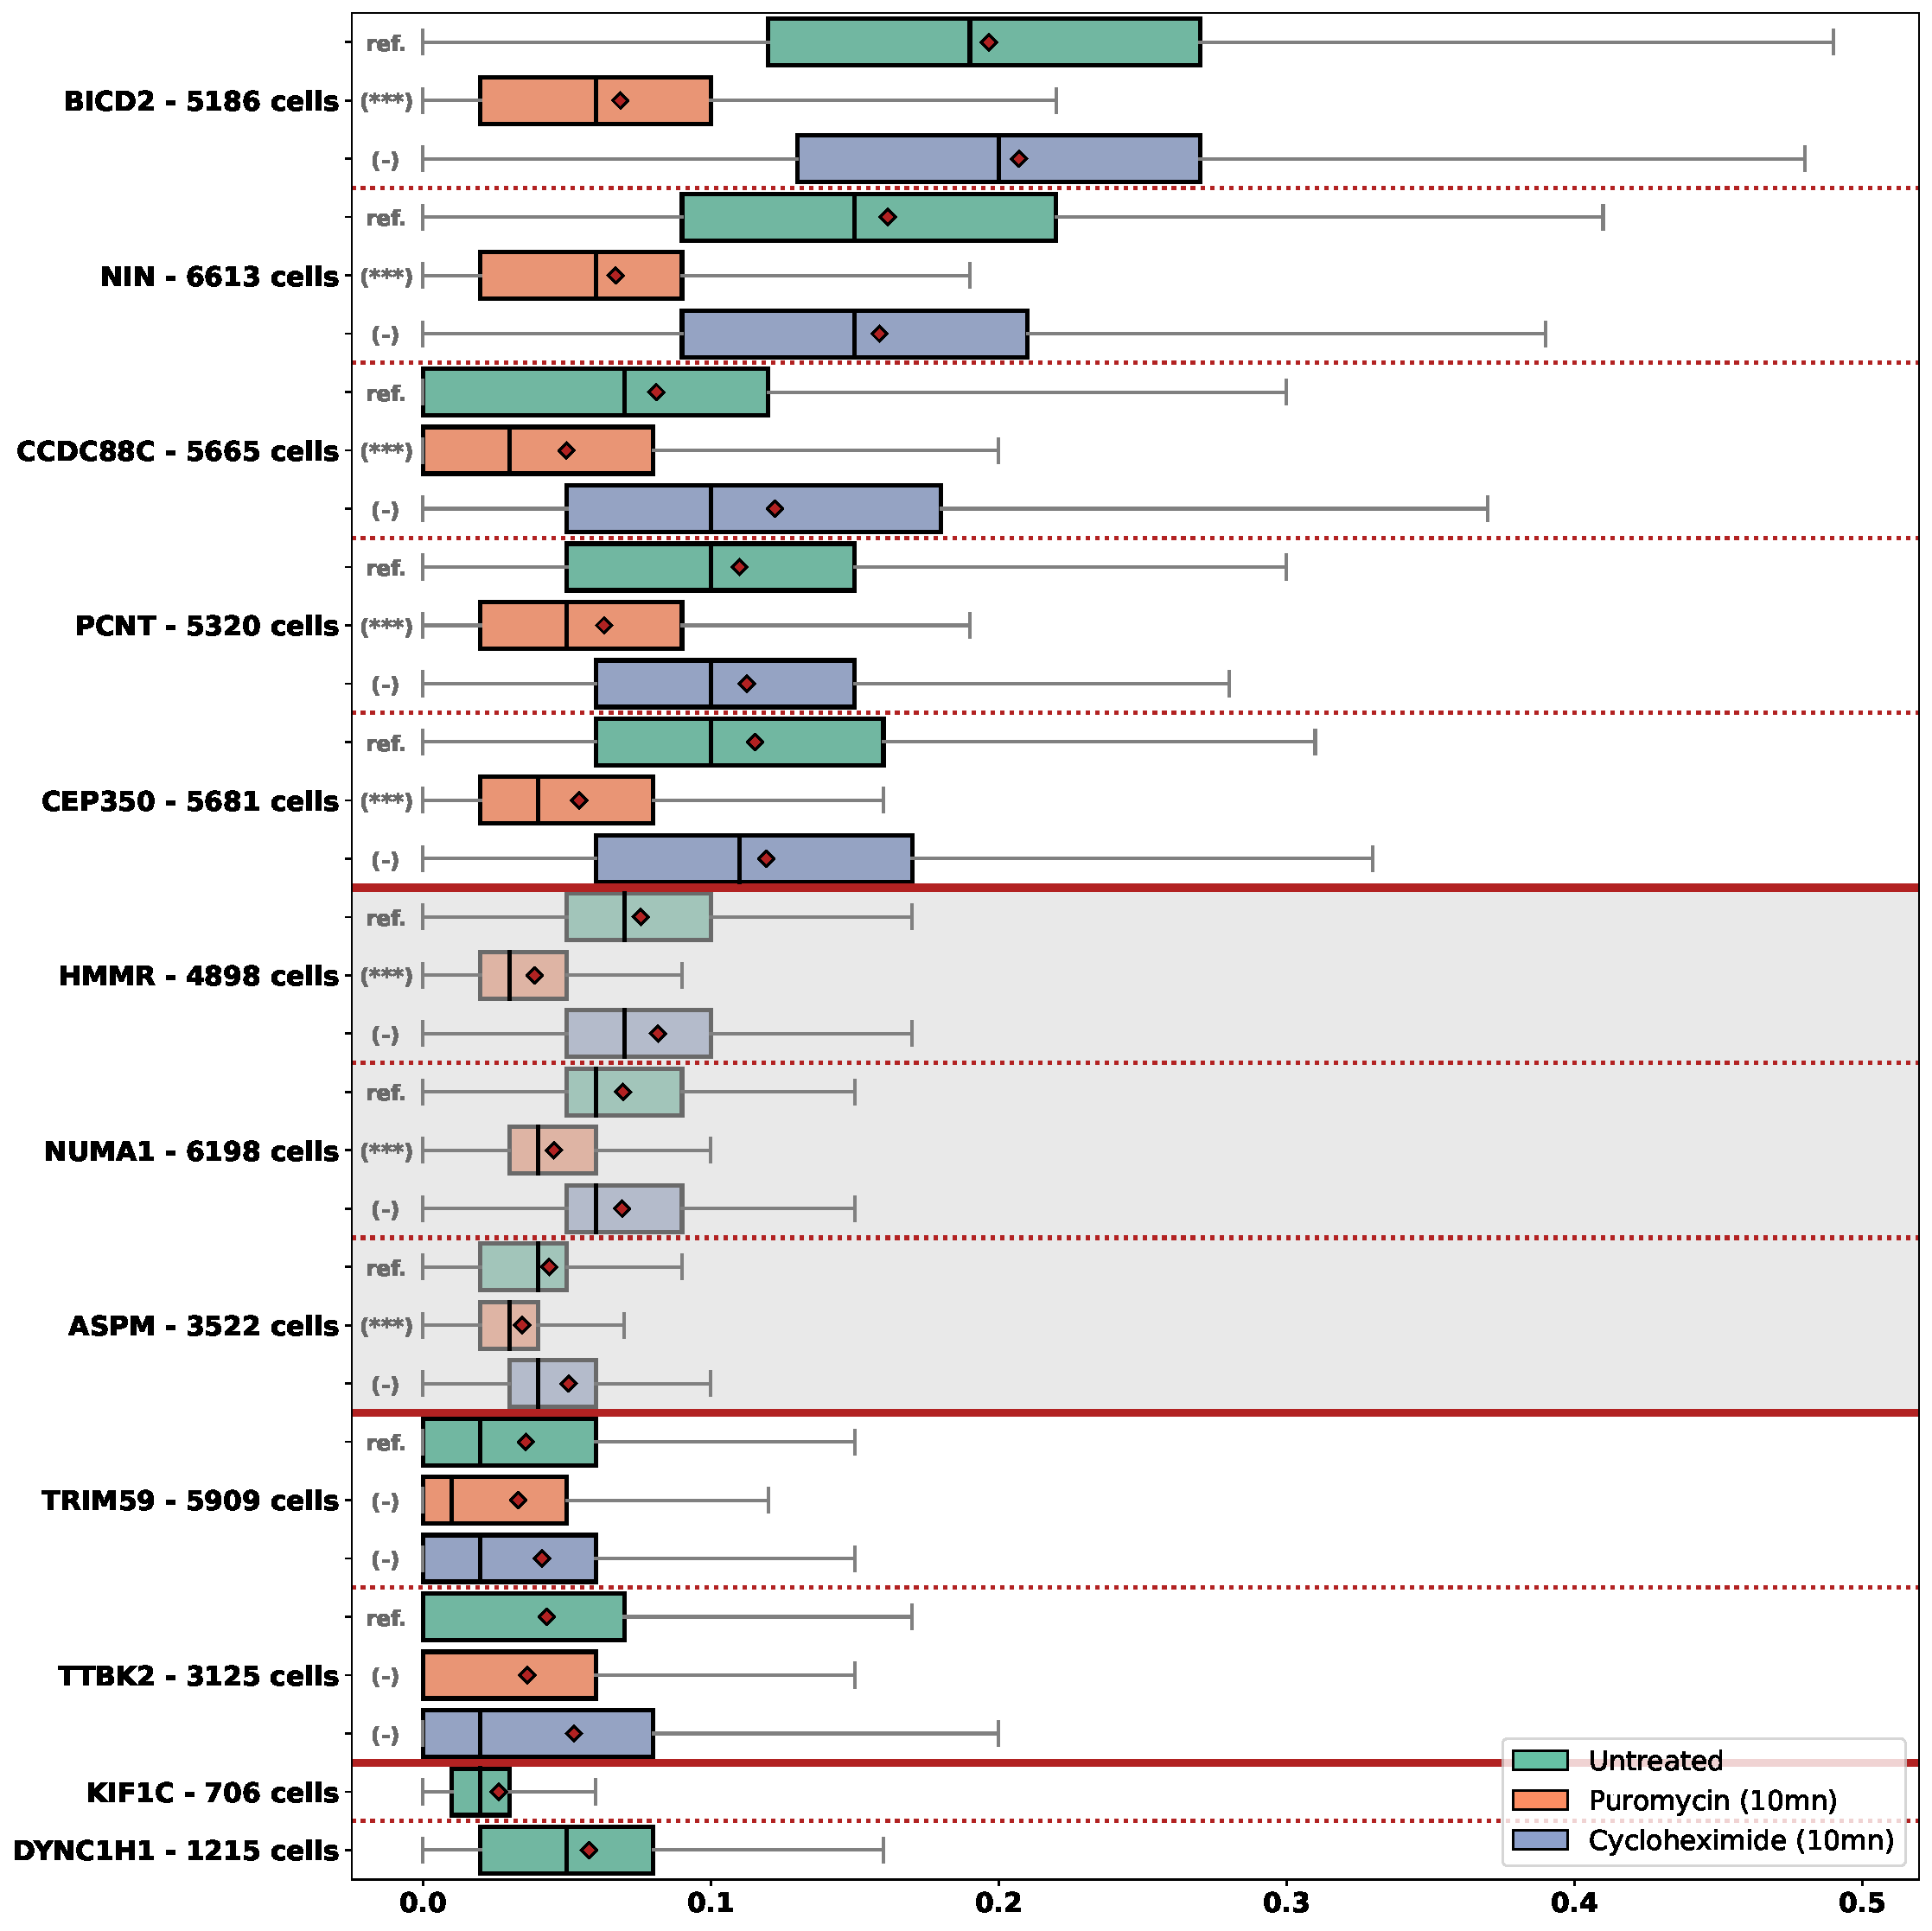
\includegraphics[width=\textwidth]{figures/chapter5/plot_rna_centrosome}
    \caption[Box plot with the proportion of centrosomal mRNAs]{Box plot with the proportion of centrosomal mRNAs in cells (interphase and mitotic phase), for different genes and treatments.
	Red diamonds are the mean and the \textit{whiskers} equal 1.5 the interquartile range.
	HMMR, NUMA1 and ASPM (in \textit{gray}) are endogenous mRNAs, the rest are BAC-transcribed mRNAs.
	TRIM59, TTBK2, KIF1C and DYNC1H1 are used as control mRNAs.
	A one-sided Welch’s t-test is used to evaluate significance (***: p-value < 0.001)}
    \label{fig:plot_rna_centrosome}
\end{figure}

My contribution in~\cite{safieddine_choreography_2021} was to quantify centrosomal \ac{mRNA} localization.
Among the centrosomal protein-coding genes analyzed, we found 8 \ac{mRNA}s accumulating in centrosome's neighborhood: BICD2, NIN, CCDC88C, PCNT, CEP350, HMMR, NUMA1 and ASPM.
I designed a quantitative pipeline to process a high-content screening dataset and compute the proportion of \ac{mRNA}s detected around a centrosome.
The results are reported in Figure~\ref{fig:plot_rna_centrosome}.
In addition to the centrosomal transcripts, I also processed several control genes without the studied pattern.
While TRIM59 and TTBK2 present no specific localization pattern, KIF1C and DYNC1H1 are respectively and frequently identified with protrusion and foci patterns (see Section~\ref{sec:general_pattern_recognition}).

Two main observations can be drawn from this plot.
First, most of the centrosomal \ac{mRNA}s display a higher proportion of transcripts around the centrosomes: from 4.4\% (ASPM) to 19.7\% (BICD2), against 4.0\% for the control genes, in average.
These results already illustrate a limitation of my quantification, since the gene ASPM displayed a lower proportion of centrosomal \ac{mRNA}s than our control DYNC1H1 (5.8\% in average).
DYNC1H1 transcripts accumulate in foci close to the nucleus can thus can be easily confused with a centrosomal pattern.

Importantly, we can observe in Figure~\ref{fig:plot_rna_centrosome}, that a while a Puromycin treatment resulted in a drop of centrosomal \ac{mRNA}s localization, Cycloheximide treatment did not.
Similarly to the translation factories, it suggests that the centrosomal pattern is driven by the presence of nascent peptide chains.

\subsubsection{A cell cycle regulated localization}

In order to get a more detailed view of this RNA localization, we implemented an image analysis approach to obtain the cell-cycle of each cell (interphase and early/late mitosis).
Five \ac{mRNA}s exhibited a centrosomal localization pattern during interphase and early mitosis: HMMR, BICD2, CEP350, PCNT and NIN.
In addition, HMMR was the only gene whose \ac{mRNA}s and proteins co-localized at cytokinetic bridge in telophase.
Lastly, ASPM and NUMA1 localized only during mitosis and CCDC88C in interphase.
However, while NUMA1 \ac{mRNA}s localized during early mitosis (prophase and prometaphase), a centrosomal accumulation of ASPM \ac{mRNA}s can be observed for every mitotic phase.
All in all, these results reveal an elegant \emph{choreography} of \ac{mRNA} localization, cell cycle regulated and translation driven.

\section{The key role of KIF1C in protrusion pattern}
\label{sec:protrusion}

In~\cite{pichon_kinesin_2021}, I could take full benefit from the developed analysis pipeline to extract quantitative results from a \ac{smFISH} high content screening study.
My contribution for this study, was the quantification of a protrusion pattern manifested by the accumulation of \ac{mRNA}s in cell extensions.

\subsection{KIF1C and protrusion mRNAs}
\label{subsec:introduction_protrusion}

Three \ac{RNA} transport mechanisms are reported in the literature~\cite{Medioni_2012, Bovaird_2018}:

\begin{enumerate}
	\setlength\itemsep{0.1em}
	\item a localized protection from \ac{RNA} degradation
	\item a random diffusion coupled with a targeted entrapment
	\item an active \ac{RNA} transport along the cytoskeleton, with specific motor proteins
\end{enumerate}

\noindent
In this section, we focus on the active transport mechanism.
As an example, in vertebrates, the $\beta$-actin \ac{mRNA} has a \emph{zipcode} sequence that the \ac{RBP} ZBP1 will recognize, hence allowing the transport of the \ac{mRNA} molecule along microtubules and actin filaments~\cite{Oleynikov_2003}.

More specifically, we investigated the role of the kinesin KIF1C that accumulates in cell protrusion (see Figure~\ref{fig:heatmap_racha}) and encodes a microtubule motor protein.
This protein interacts with a specific group of \ac{mRNA}s defined as APC-dependent (they require the APC protein to localize~\cite{wang_extracellular_2017}).
KIF1C protein binds a subset of these \ac{mRNA}s and transports them to cell extensions where they localize in RNA foci: NET1, TRAK2 and RAB13 .
Interestingly, this kinesin protein also actively transports its own transcripts to protrusions.

Finally, we demonstrated that KIF1C is needed to transport these APC-dependent \ac{mRNA}s to protrusions along microtubules and to form their foci.
Indeed, we did not observe these foci in cell extensions when the KIF1C protein is absent.
These results suggest a dual function of KIF1C as microtubule motor and ''\ac{mRNA} anchoring module promoting clustering''~\cite{pichon_kinesin_2021}.

\subsection{Quantification of peripheral mRNAs}
\label{subsec:materials_results_protrusion}

This study was an opportunity to exploit a proven FISH-quant v2 and to scale a quantitative analysis that characterizes protrusion \ac{RNA}s from HeLa cells.
I identified 27,644 individual cells, detecting \ac{mRNA}s from 40 different genes, including KIF1C, APC-dependent \ac{mRNA}s and control transcripts.
For every cell, I performed an automated spot detection, nucleus and cell segmentation, from 2D projected images.
I compute RDI Calculator features from~\cite{stueland_rdi_2019}, especially the peripheral distribution index that measures how close the \ac{RNA}s localize to the cell periphery (see Section~\ref{subsec:expert_features}).
The greater this index, the more concentrated in the protrusion are the transcripts.

\begin{figure}[]
    \centering
    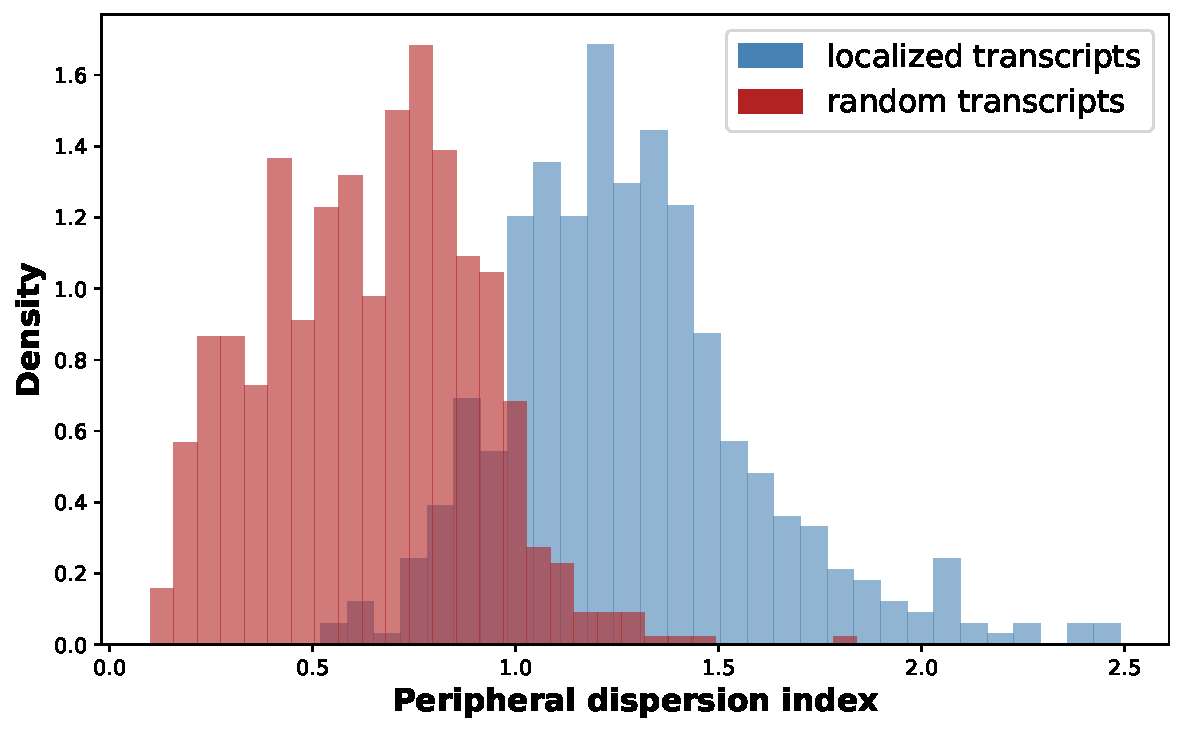
\includegraphics[width=\textwidth]{figures/chapter5/helacentrin_distribution_pdi}
    \caption[Histogram of the peripheral distribution index]{Histogram of the peripheral distribution index for two group of transcripts.
	Localized transcripts include: KIF1C, TRAK2 and NET1.
	Control transcripts include NEK9, NIN, NPM1, OBSL1, OLA1, PAX2, PKHD1, RGS14, SMAD7 and SPAST}
    \label{fig:xavier_pdi}
\end{figure}

In Figure~\ref{fig:xavier_pdi}, I compared two groups of transcripts: KIF1C, TRAK2 and NET1, three \ac{mRNA}s that bind to KIF1C protein for active transport to the protrusions, and a control group unrelated to KIF1C.
For the peripheral distribution index, a completely random distribution has a value of 1.
Here, as expected, the protrusion \ac{mRNA}s exhibited a biased spatial distribution toward the cell extensions.

\section{Conclusion}
\label{sec:conclusion_chapter5}

In this chapter, I present several applications of FISH-quant v2.
Based on several high content screens in HeLa cell, I performed large scale quantitative analyses to answer question centered around RNA localization and local translation.
In total, several dozens of transcripts were analyzed across 100,000 individual cells and hundreds of fluorescent bioimages.

In~\cite{CHOUAIB_2020}, I provided quantifications highlighting the high level of heterogeneity in \ac{mRNA}s localization, both on the population as well as the single-cell level.
The developed classification pipeline enabled the identification of complex RNA localization patterns: intranuclear, nuclear edge, perinuclear, foci and protrusion.
We showed that the foci pattern is caused by two distinct biological processes: first, RNA storage in \ac{P-bodies} and second, translation factories, where RNAs are efficiently translated
By extrapolating to the 20,000 human genes, we could expect to find a few hundred of translation factory structures in a cell.
Remarkably, such phenomenon of locally targeted translation is observed for other localization patterns.
For some cases, this localization even seems to be translation dependent and tends to disappear if the nascent protein synthesis is inhibited.

In~\cite{safieddine_choreography_2021}, a second set of localized transcripts was analyzed with spatial and temporal dynamics.
I characterized \ac{mRNA}s with a centrosomal localization.
This pattern presents a temporal dynamic in addition to be translation dependent.
Cell cycle regulates the choreography and the localization of different \ac{mRNA}s around the centrosomes.

In~\cite{pichon_kinesin_2021}, we confirmed the importance of the KIF1C motor protein in the transport of some APC-dependent transcripts to cell extensions.
Surprisingly, this proteins also bind its own \ac{mRNA}s along microtubules which suggests the existence of a positive feedback loop to locally enrich cell protrusion with the needed \ac{mRNA}s.

Taken together, our data suggest that even in a simple system such as HeLa cells, translation might be compartmentalized to a much higher degree and with a finer granularity than anticipated.
Our analysis reveals spatial and temporal dynamics as well as complex mechanisms to regulate the metabolism of nascent proteins.
Robust quantitative and numerical methods are needed more than ever to address these complexity and volume of interactions.